% !TeX document-id = {fb8a2ef5-cdaf-49da-b79d-0a8152e677cd}
% !TeX TS-program = XeLaTeX
\documentclass[a4paper,12pt]{report}

% polyglossia should go first!
\usepackage{polyglossia} % multi-language support
\setmainlanguage{russian}
\setotherlanguage{english}

\usepackage{amsmath} % math symbols, new environments and stuff
\usepackage{unicode-math} % for changing math font and unicode symbols
\usepackage[style=english]{csquotes} % fancy quoting
\usepackage{microtype} % for better font rendering
\usepackage{hyperref} % for refs and URLs
\usepackage{graphicx} % for images (and title page)
\usepackage{geometry} % for margins in title page
\usepackage{tabu} % for tabulars (and title page)
\usepackage[section]{placeins} % for float barriers
\usepackage{titlesec} % for section break hooks
\usepackage{listings} % for listings 
\usepackage{upquote} % for good-looking quotes in source code (used for custom languages)
\usepackage{xcolor} % colors!
\usepackage{enumitem} % for unboxed description labels (long ones)
\usepackage{caption}

\defaultfontfeatures{Mapping=tex-text} % for converting "--" and "---"
\setmainfont{CMU Serif}
\setsansfont{CMU Sans Serif}
\setmonofont{CMU Typewriter Text}
\setmathfont{XITS Math}
\MakeOuterQuote{"} % enable auto-quotation

% new page and barrier after section, also phantom section after clearpage for
% hyperref to get right page.
% clearpage also outputs all active floats:
\newcommand{\sectionbreak}{\phantomsection}
\newcommand{\subsectionbreak}{\FloatBarrier}
\renewcommand{\thesection}{\arabic{section}} % no chapters
\numberwithin{equation}{section}
%\usetikzlibrary{shapes,arrows,trees}

\newcommand{\itemtt}[1][]{\item[\texttt{#1}:]} % tt-ed items (for protocol descriptions)

\definecolor{bluekeywords}{rgb}{0.13,0.13,1}
\definecolor{greencomments}{rgb}{0,0.5,0}
\definecolor{turqusnumbers}{rgb}{0.17,0.57,0.69}
\definecolor{redstrings}{rgb}{0.5,0,0}
\setmonofont{Consolas} %to be used with XeLaTeX or LuaLaTeX
\definecolor{bluekeywords}{rgb}{0,0,1}
\definecolor{greencomments}{rgb}{0,0.5,0}
\definecolor{redstrings}{rgb}{0.64,0.08,0.08}
\definecolor{xmlcomments}{rgb}{0.5,0.5,0.5}
\definecolor{types}{rgb}{0.17,0.57,0.68}

\lstset{language=[Sharp]C,
captionpos=b,
%numbers=left, %Nummerierung
%numberstyle=\tiny, % kleine Zeilennummern
frame=lines, % Oberhalb und unterhalb des Listings ist eine Linie
showspaces=false,
showtabs=false,
breaklines=true,
showstringspaces=false,
breakatwhitespace=true,
escapeinside={(*@}{@*)},
commentstyle=\color{greencomments},
morekeywords={partial, var, value, get, set},
keywordstyle=\color{bluekeywords},
stringstyle=\color{redstrings},
basicstyle=\ttfamily\small,
}

\lstset{
  numbers=left,
  numberstyle=\scriptsize,
  basicstyle=\ttfamily\scriptsize,
  columns=fullflexible,
  keepspaces, % for spaces in unicode text!
  captionpos=b
}
\renewcommand{\lstlistingname}{Листинг}

\date{\today}

\makeatletter
\let\thetitle\@title
\let\theauthor\@author
\let\thedate\@date
\makeatother

\makeatletter
\AtBeginDocument{%
    \expandafter\renewcommand\expandafter\subsection\expandafter{%
        \expandafter\@fb@secFB\subsection
    }%
}
\makeatother

\begin{document}

\tableofcontents

\clearpage
\section*{Глоссарий}
\begin{itemize}
  \item комплекс
  \item сус
  \item сбн
  \item су  
  \item 
  \item задача
  \item пользователь
  \item вычислительный узел
  \item 
  \item x?
  \item 
  \item 
\end{itemize}

\clearpage
\section*{Введение}

\clearpage
\section{Аналитический раздел}
\subsection{Введение}
В данном разделе выполняется анализ предметной области.
Результаты анализа представляются в виде диаграм прецедентов и деятельности.

\subsection{Возможные прецеденты}
Комплекс при его работе предоставляет пользователю следующие варианты использования:
\begin{itemize}
  \item регистрация пользователя;
  \item авторизация пользователя;
  \item постановка задачи на исполнение;
  \item просмотр статуса задачи;
  \item отмена задачи.
\end{itemize}

Диаграмма этих и дополнительных служебных прецедентов приведена на рис.~\ref{fig:prec-common}.

\begin{figure}[b]
  \centering
  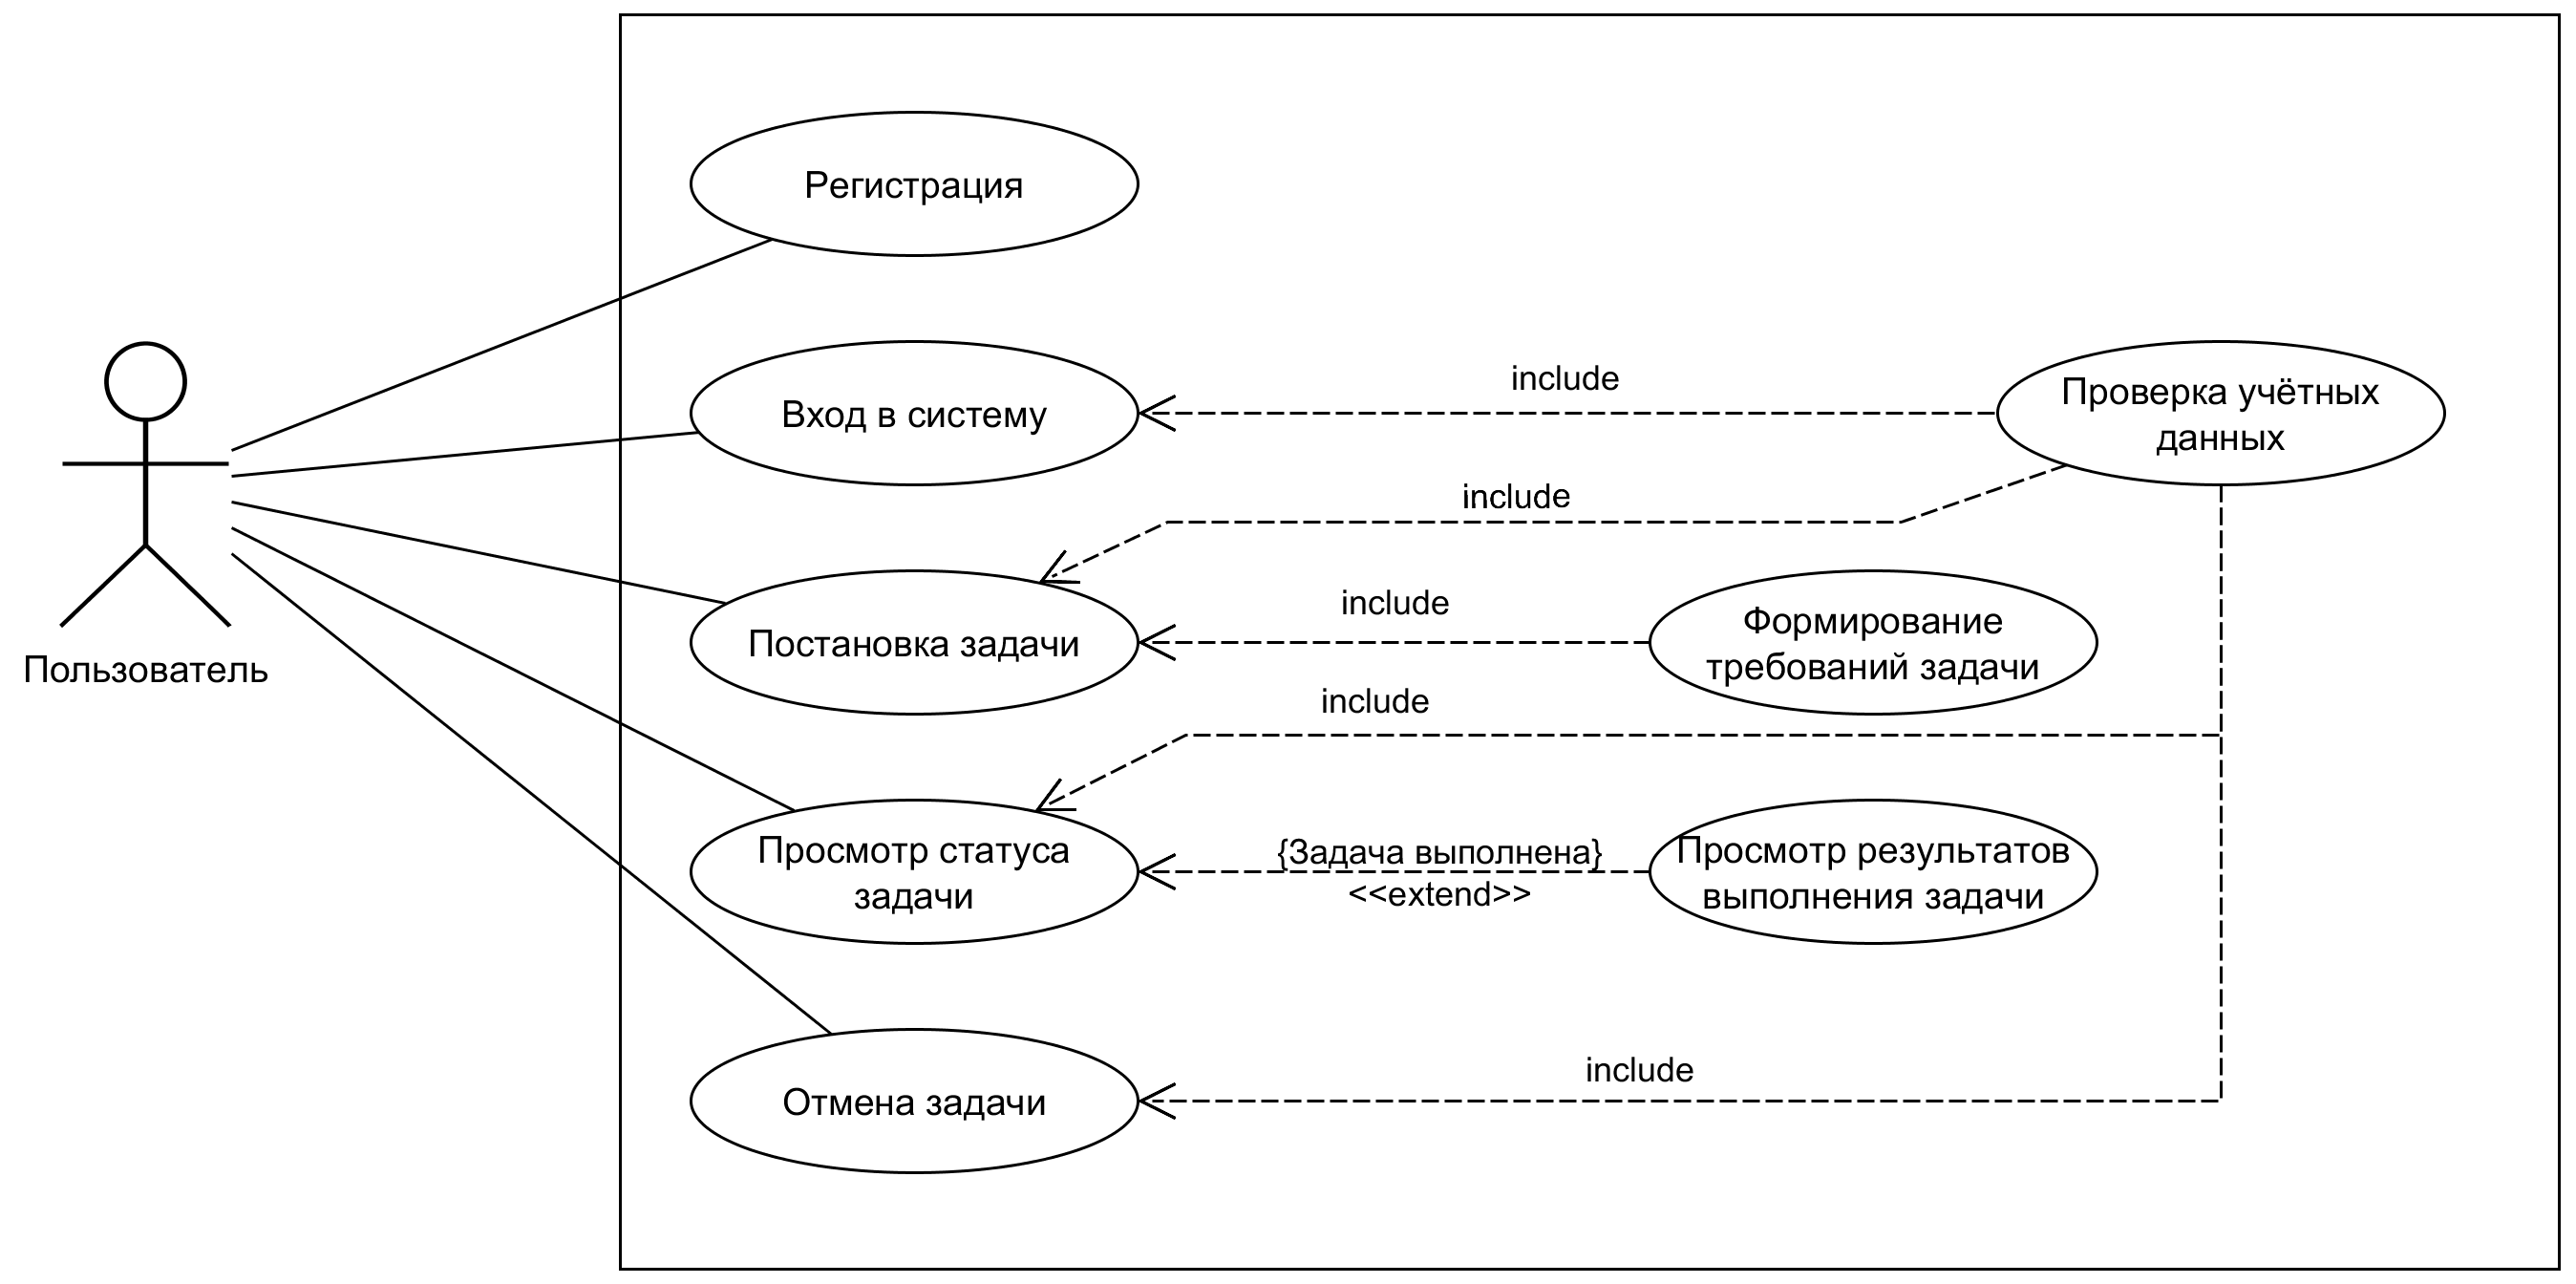
\includegraphics[width=.9\linewidth]{diagrams/common/usecase}
  \caption{Диаграмма прецедентов всеего комплекса в целом}
  \label{fig:prec-common}
\end{figure}

С учётом требований к разделению внутреннего функционала комплекса, диаграмма прецедентов на рис.~\ref{fig:prec-common}
расщепляется на набор диаграмм, соответствующих каждой из выделенных подсистем.
Соответствующие диаграммы приведены на рисунках~\ref{fig:prec-session},\ref{fig:prec-logic},\ref{fig:prec-balancer}.

\begin{figure}
  \centering
  \begin{minipage}{.49\linewidth}
    \centering
    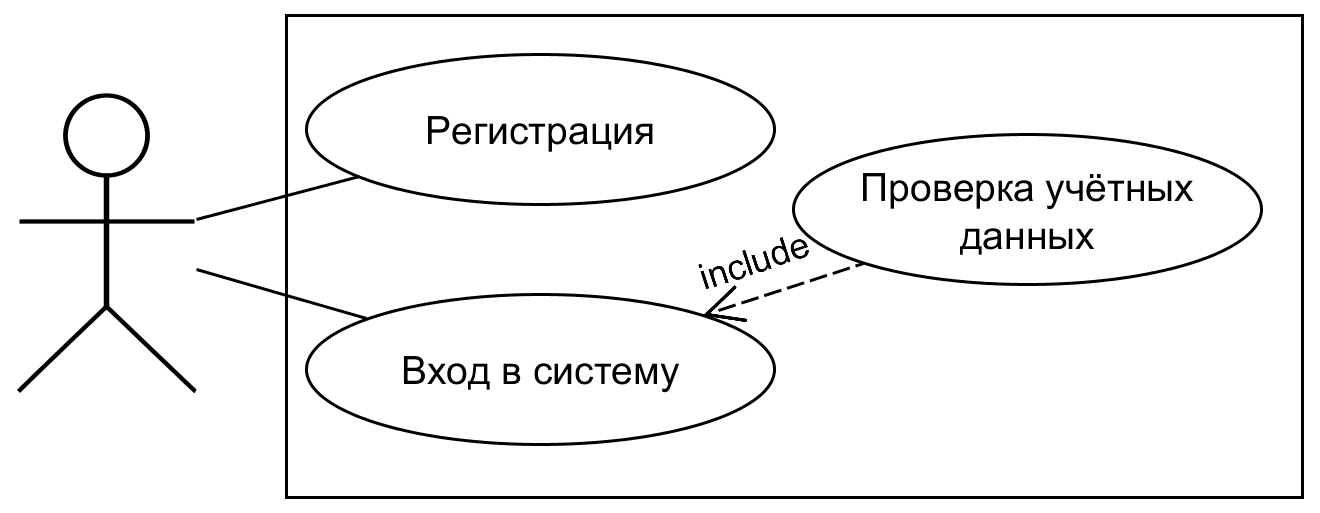
\includegraphics[width=\linewidth]{diagrams/session/usecase}
    \caption{Диаграмма прецедентов СУС}
    \label{fig:prec-session}
  \end{minipage}
  \hfill
  \begin{minipage}{.49\linewidth}
    \centering
    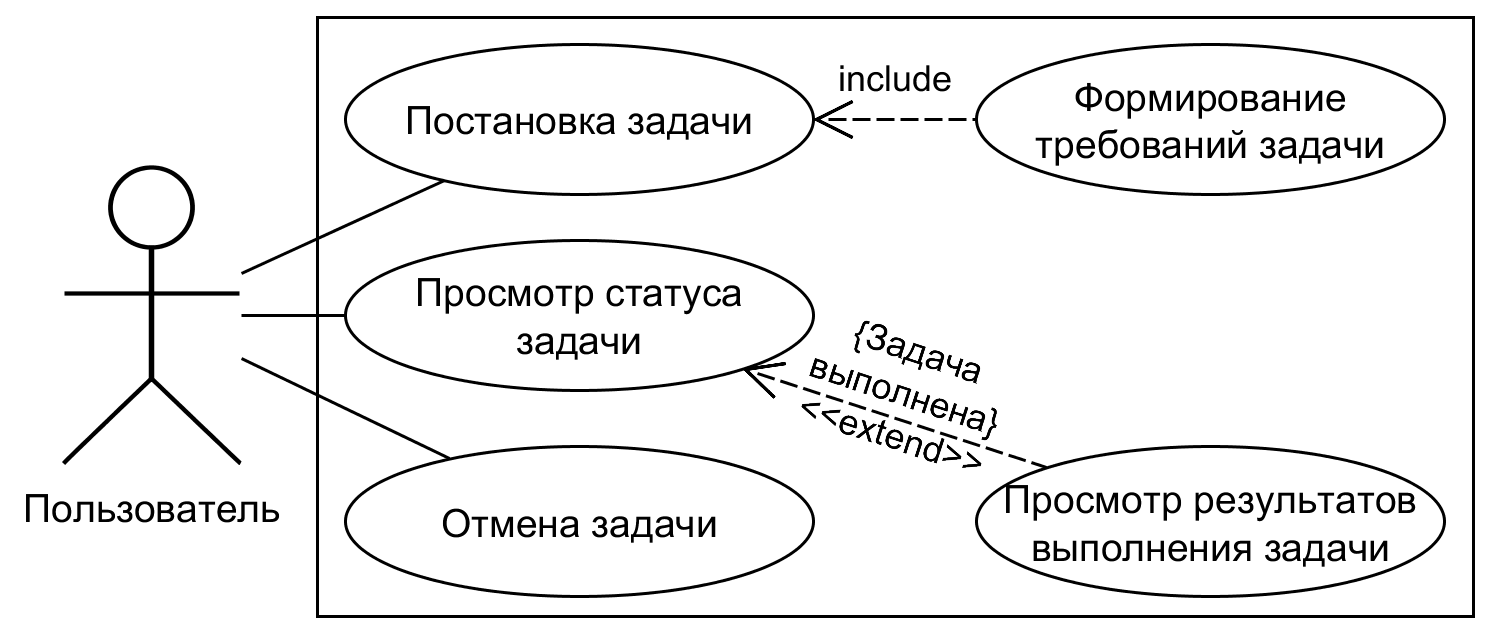
\includegraphics[width=\linewidth]{diagrams/logic/usecase}
    \caption{Диаграмма прецедентов СУ}
    \label{fig:prec-logic}
  \end{minipage}  
\end{figure}

\begin{figure}
  \centering
  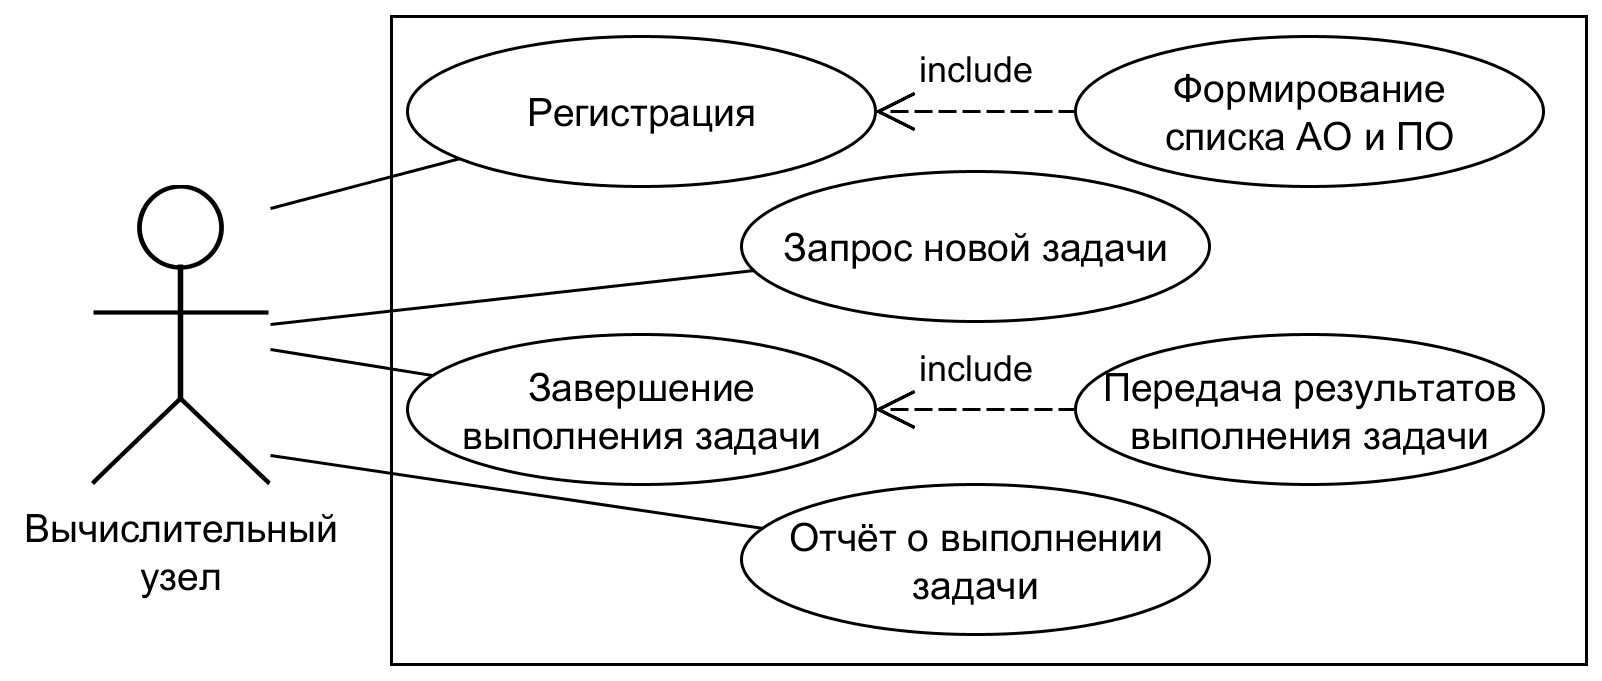
\includegraphics[width=.6\linewidth]{diagrams/balancer/usecase}
  \caption{Диаграмма прецедентов СБН}
  \label{fig:prec-balancer}
\end{figure}

\subsection{Осуществляемая деятельность}
Прецеденты, описанные в предыдущем пункте, отвечают определённой деятельности.
Диаграмма деятельности на рис.~\ref{fig:act-common} описывает полный процесс взаимодействия пользователя с комплексом.

С учётом требований к разделению внутреннего функционала комплекса, диаграмма деятельности на рис.~\ref{fig:act-common}
расщепляется на набор диаграмм, соответствующих определённым подсистемам из выделенных.

Диаграммы действий прецедентов подсистемы управления сессией "регистрация" и "вход в систему" приведены на рисунках~\ref{fig:act-register} и~\ref{fig:act-auth} соответственно.

Диаграммы действий прецедентов системы балансировки нагрузки "регистрация", "запрос новой задачи" и "завершение выполнения задачи" приведены на рисунках~\ref{fig:bal-register},~\ref{fig:bal-request} и~\ref{fig:bal-submit} соответственно.

Диаграммы действий прецедентов системы управления "постановка задачи" и "просмотр статсуа задачи" приведены на рисунках~\ref{fig:logic-place} и~\ref{fig:logic-view} соответственно.

\begin{figure}[h]
  \centering
  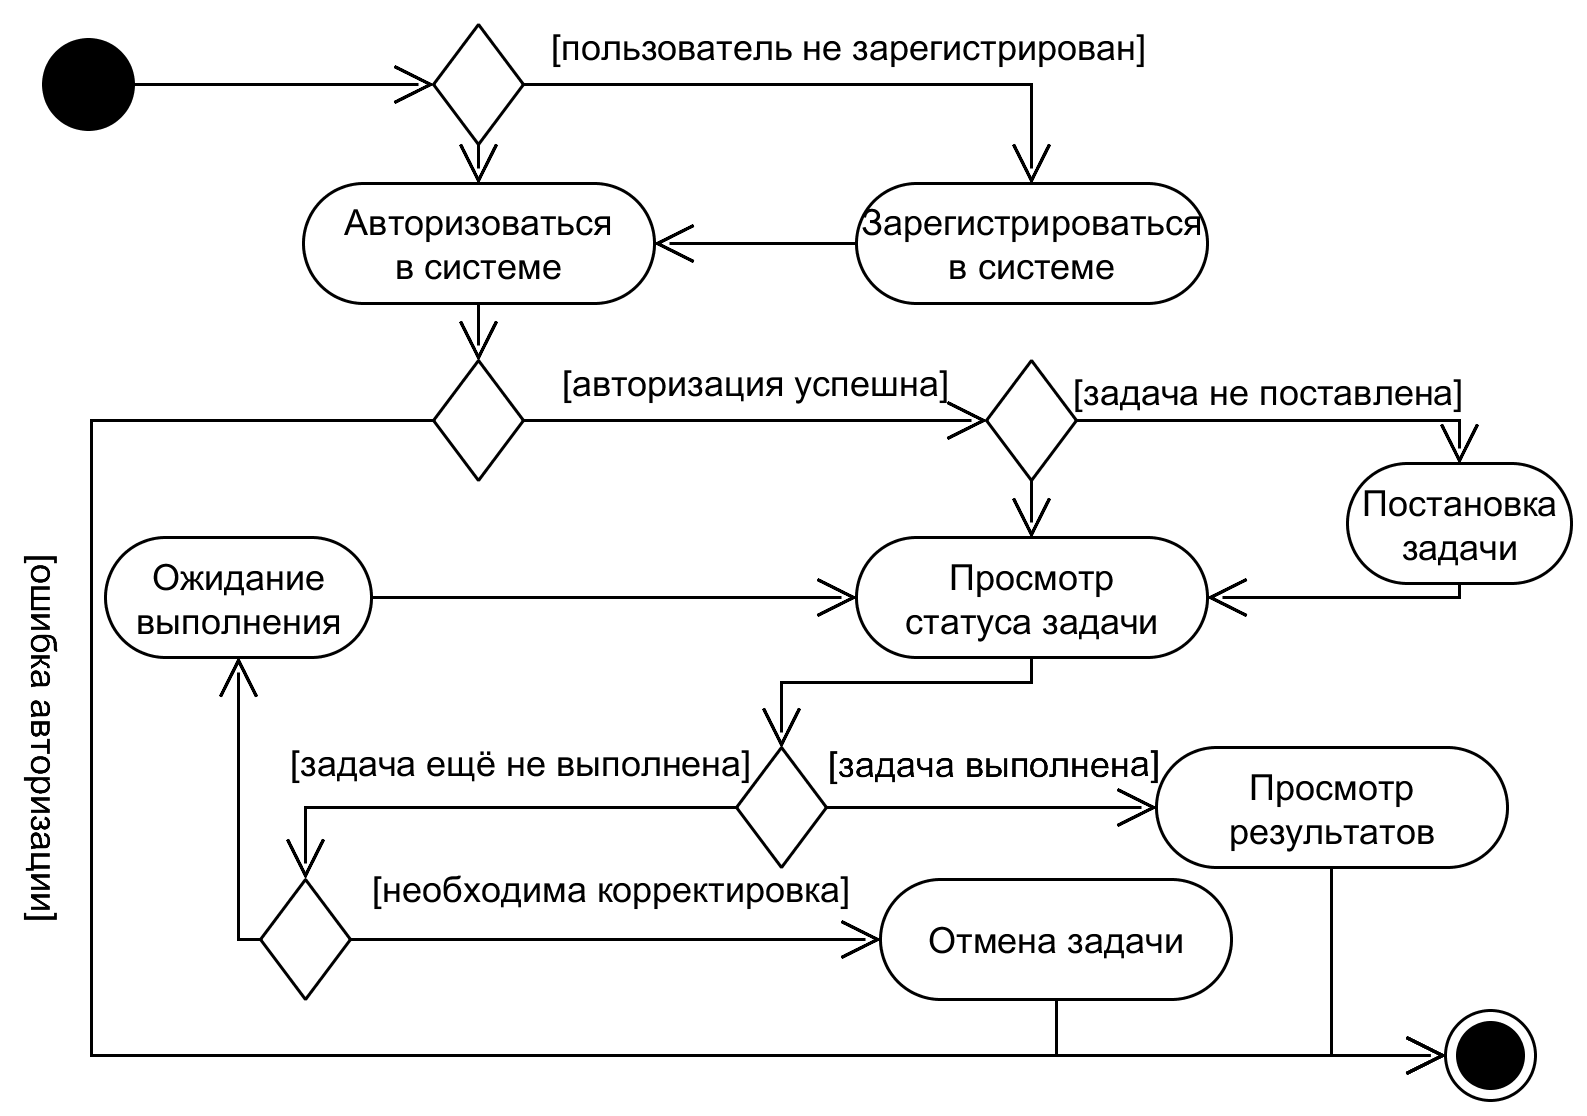
\includegraphics[width=.9\linewidth]{diagrams/common/activity}
  \caption{Диаграмма действий прецедента "общая деятельность" для системы в целом}
  \label{fig:act-common}
\end{figure}

\begin{figure}
  \centering
  \begin{minipage}{.43\linewidth}
    \centering
    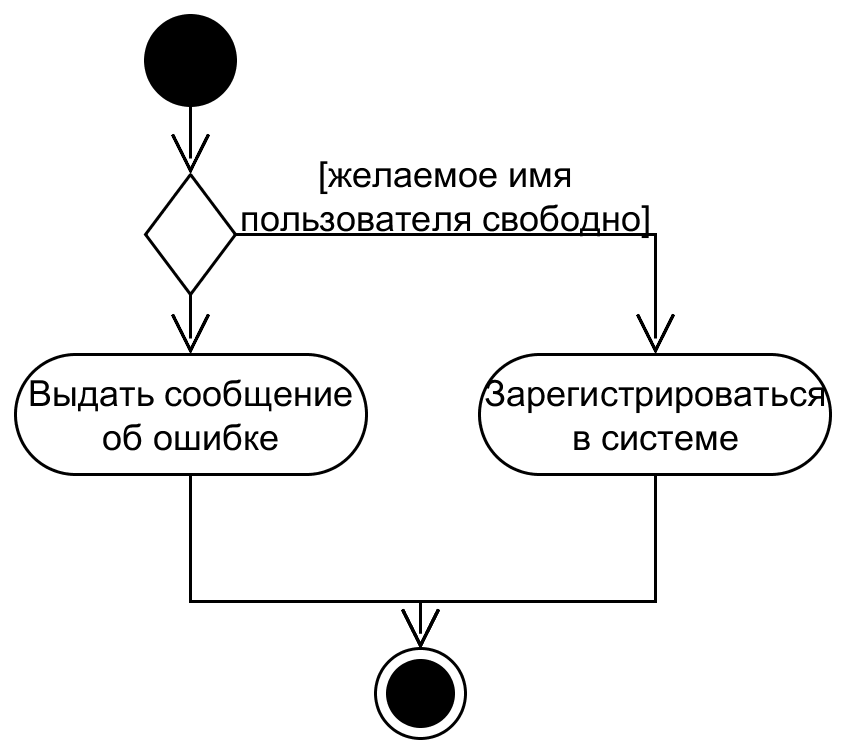
\includegraphics[width=\linewidth]{diagrams/session/activity-register}
    \caption{Диаграмма действий прецедента "регистрация" СУС}
    \label{fig:act-register}
  \end{minipage}
  \hfill
  \begin{minipage}{.53\linewidth}
    \centering
    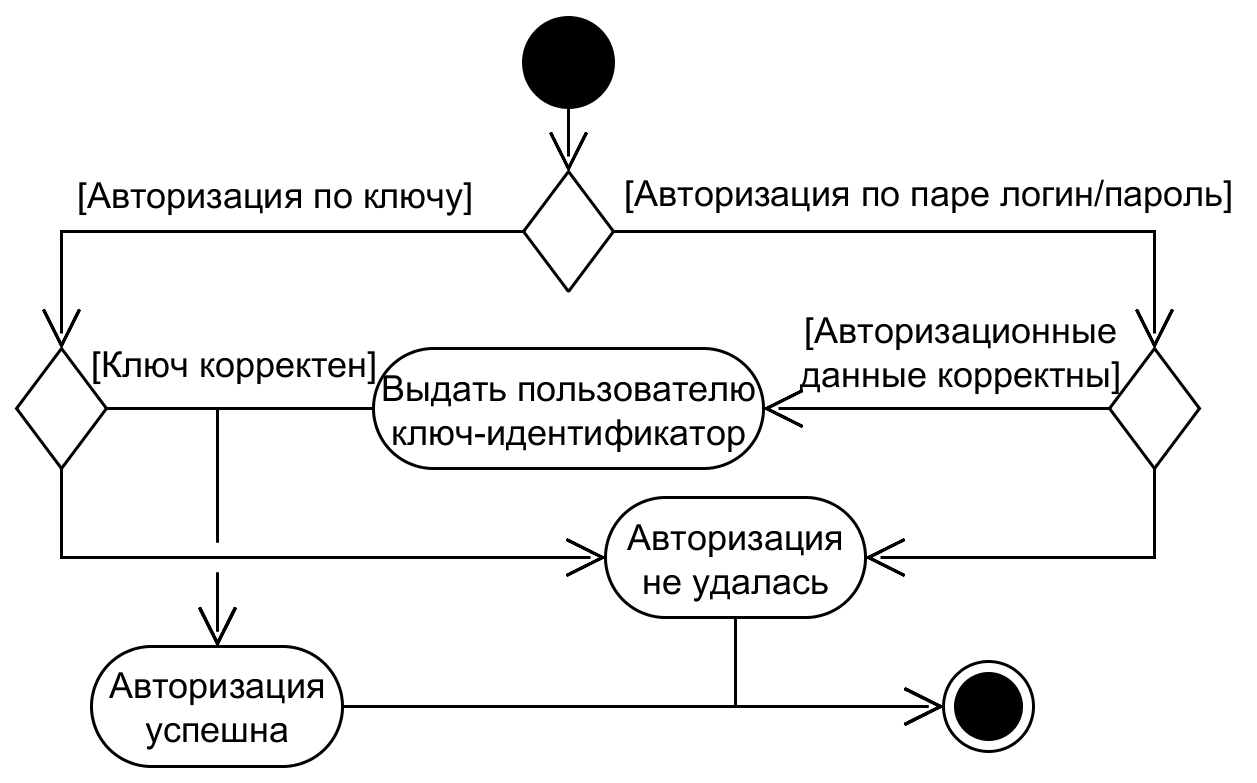
\includegraphics[width=\linewidth]{diagrams/session/activity-authorize}
    \caption{Диаграмма действий прецедента "вход в систему" СУС}
    \label{fig:act-auth}
  \end{minipage}  
\end{figure}

\begin{figure}  
  \centering
  \begin{minipage}{.49\linewidth}
    \centering
    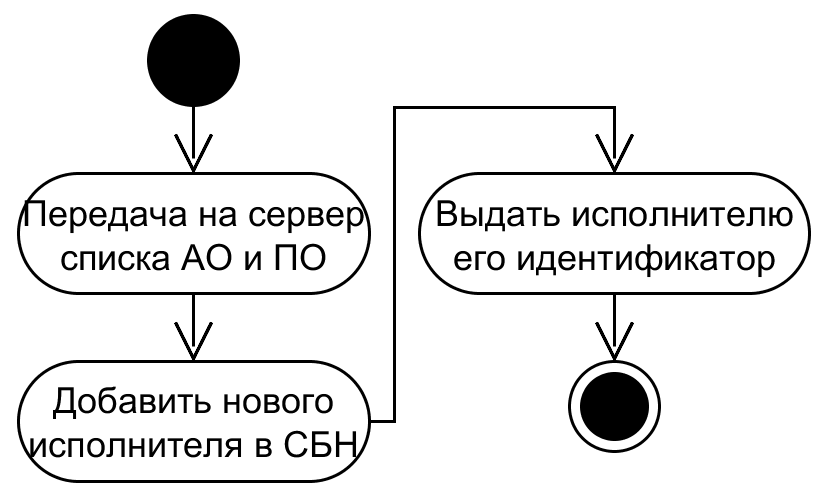
\includegraphics[width=\linewidth]{diagrams/balancer/activity-register}
    \caption{Диаграмма действий прецедента "регистрация" СБН}
    \label{fig:bal-register}
  \end{minipage}
  \hfill
  \begin{minipage}{.49\linewidth}
    \centering
    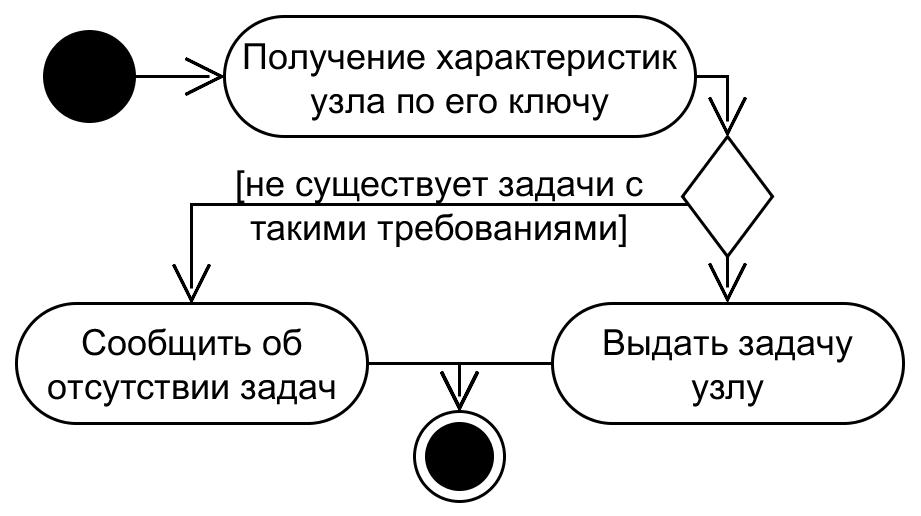
\includegraphics[width=\linewidth]{diagrams/balancer/activity-request}
    \caption{Диаграмма действий прецедента "запрос новой задачи" СБН}
    \label{fig:bal-request}
  \end{minipage}  
\end{figure}

\begin{figure}  
  \centering
  \begin{minipage}{.49\linewidth}
    \centering
    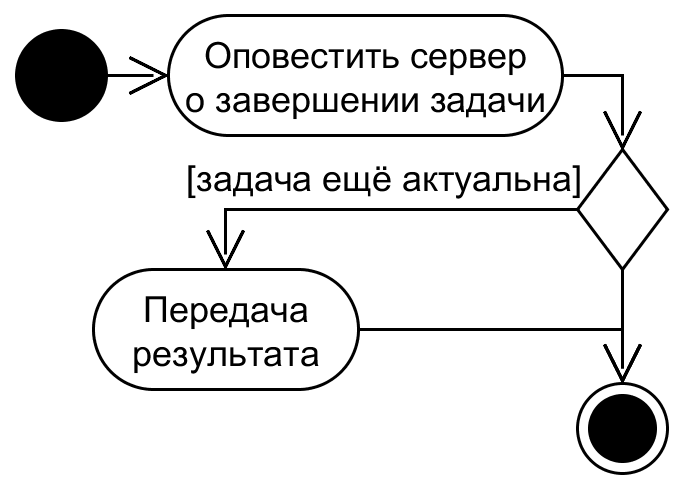
\includegraphics[width=\linewidth]{diagrams/balancer/activity-submit}
    \caption{Диаграмма действий прецедента "завершение выполнения задачи" СБН}
    \label{fig:bal-submit}
  \end{minipage} 
  \hfill
  \begin{minipage}{.49\linewidth}
    \centering
    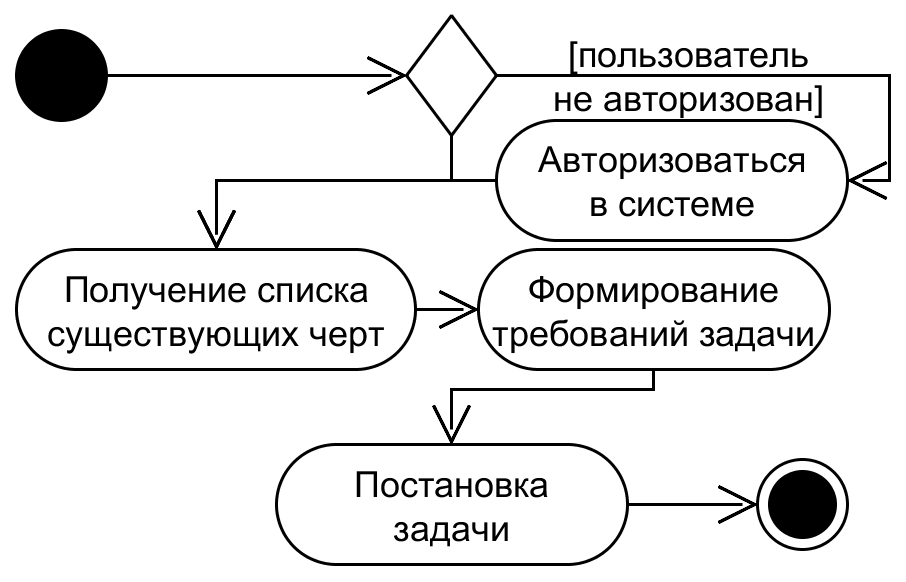
\includegraphics[width=\linewidth]{diagrams/logic/activity-place}
    \caption{Диаграмма действий прецедента "постановка задачи" СУ}
    \label{fig:logic-place}
  \end{minipage} 
\end{figure}

\begin{figure}
  \centering
  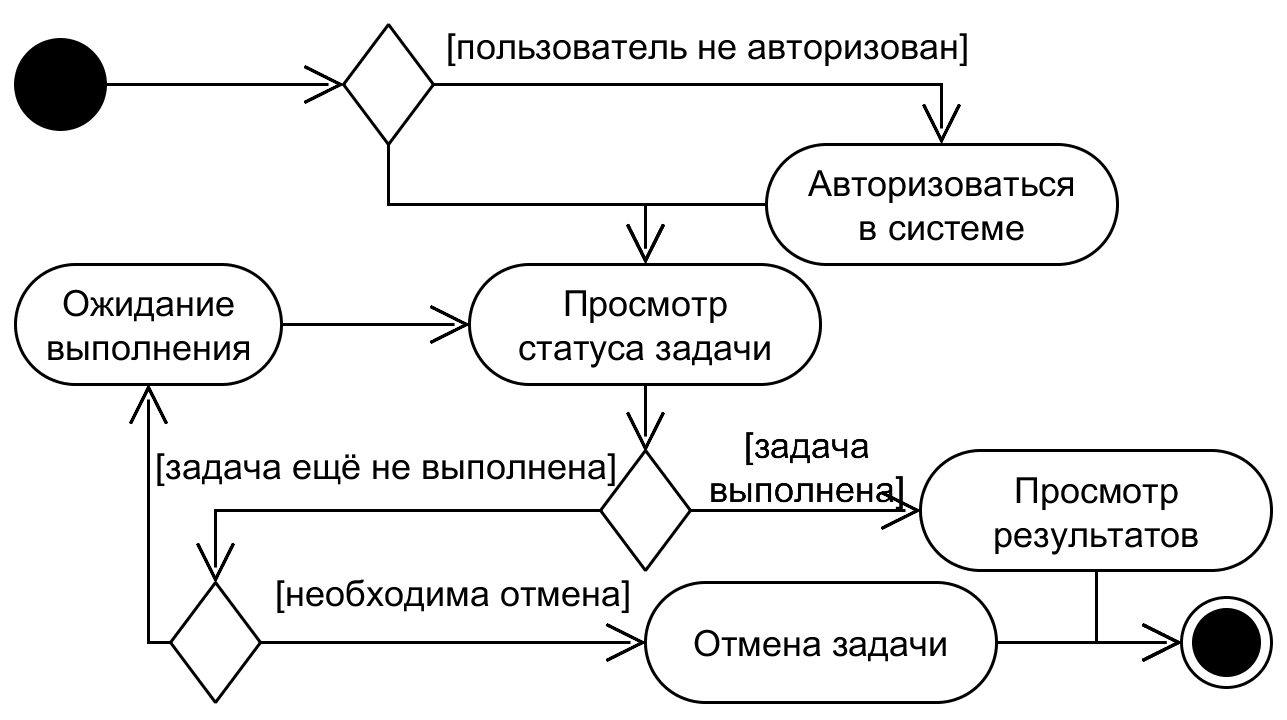
\includegraphics[width=\linewidth]{diagrams/logic/activity-view}
  \caption{Диаграмма действий прецедента "просмотр статсуа задачи" СУ}
  \label{fig:logic-view}
\end{figure}

\subsection{Вывод}
В данном разделе были приведены диаграммы, описывающие функционал основных узлов системы.
Данный анализ в дальнейшем используется для более строгой формализации функционала подсистем.

\clearpage
\section{Конструкторский раздел}
\subsection{Введение}
В данном разделе приводятся результаты проектирования системы.
С применением UML-диаграмм описывается общая структура комплекса и требуемый функционал отдельных узлов системы.

\subsection{Общая структура системы}
Для того, чтобы удовлетворить требованиям по предоставлению механизма деградации функциональности,
а также для упрощения процесса разработки, комплекс должна быть разделена на отдельные слабосвязанные элементы.

\subsection{Система мониторинга}
Задача данной подсистемы -- отслеживание топологии сети.
Все узлы комплекса должны оповещать СМ о своём статусе работы, 
и любой узел может получить от комплекса список активных в данный момент узлов.

Невозможность любой другой подсистемы связаться с системой мониторинга рассматривается
как ошибка сети, нарушающая нормальное функционирование комплекса.

Исходя из требований к СМ и с учётом REST-методик, она должна предоставлять следующее API:

\begin{itemize}
  \item
  \begin{description}
    \item[Ресурс:] \url{/services}
    \item[Метод:] GET
    \item[Возвращаемое значение:] список активных сервисов
  \end{description}
  \item
  \begin{description}
    \item[Ресурс:] \url{/services/type}
    \item[Метод:] GET
    \item[Возвращаемое значение:] список активных сервисов такого типа
  \end{description}
  \item
  \begin{description}
    \item[Ресурс:] \url{/services/type}
    \item[Метод:] POST
    \item[Параметры:] port, state?
    \item[Возвращаемое значение:] сообщение об успешной регистрации сервиса и распознанный адрес сервиса
    \item[Ошибки:] отсутствует параметр 'port': HTTP 422
  \end{description}
  \item
  \begin{description}
    \item[Ресурс:] \url{/services/type/address}
    \item[Метод:] GET
    \item[Возвращаемое значение:] статусное сообщение выбранного сервиса, аннотированное временем создания
    \item[Ошибки:] сервис не найден: HTTP 404
  \end{description}
  \item
  \begin{description}
    \item[Ресурс:] \url{/services/type/address}
    \item[Метод:] PUT
    \item[Параметры:] state?
    \item[Возвращаемое значение:] сообщение об успешном обновлении статусного сообщения
  \end{description}
\end{itemize}

\subsection{Фронтэнд пользователей}
--- проверка безопасности + редирект на логику, возможно логика=апи, а здесь будет ещё и вебморда

\subsection{Фронтэнд вычислительных узлов}
Задача данной подсистемы -- перенаправление запросов от вычислительных узлов на балансировщик нагрузки.

Исходя из требований к СМ и с учётом REST-методик, она должна предоставлять следующее API:

\begin{itemize}
  \item
  \begin{description}
    \item[Ресурс:] \url{/nodes}
    \item[Метод:] POST
    \item[Параметры:] список черт вычислительного узла
    \item[Возвращаемое значение:] сообщение об успешной регистрации узла и назначенный идентификатор
  \end{description}
  \item
  \begin{description}
    \item[Ресурс:] \url{/nodes/identifier}
    \item[Метод:] PUT
    \item[Параметры:] состояние расчёта
    \item[Возвращаемое значение:] сообщение об успешном обновлении статуса
    \item[Ошибки:] узел разрегистрирован за неактивностью: HTTP 404
  \end{description}
  \item
  \begin{description}
    \item[Ресурс:] \url{/tasks/newtask}
    \item[Метод:] GET
    \item[Параметры:] идентификатор вычислительного узла
    \item[Возвращаемое значение:] пакет данных, описывающих задачу
    \item[Ошибки:] подходящих задач нет: HTTP 404
  \end{description}
  \item
  \begin{description}
    \item[Ресурс:] \url{/tasks/identifier}
    \item[Метод:] PUT
    \item[Параметры:] результат выполнения задачи
    \item[Возвращаемое значение:] сообщение об успешном приёме результата
  \end{description}
\end{itemize}
  
\subsection{Система управления сессией}
Задача данной подсистемы -- регистрация, авторизация и аутентификация пользователей в сети.

Исходя из требований к СМ и с учётом REST-методик, она должна предоставлять следующее API:

\begin{itemize}
  \item
  \begin{description}
    \item[Ресурс:] \url{/users}
    \item[Метод:] POST
    \item[Параметры:] желаемая пара логин / пароль (возможно, хешированный)
    \item[Возвращаемое значение:] сообщение об успешной регистрации пользователя
    \item[Ошибки:] пользователь с таким именем уже зарегистрирован: HTTP 403
  \end{description}
  \item
  \begin{description}
    \item[Ресурс:] \url{/users/username}
    \item[Метод:] GET
    \item[Параметры:] пароль (возможно, хешированный)
    \item[Возвращаемое значение:] сгенерированный ключ доступа
    \item[Ошибки:] некорректная пара логин / пароль: HTTP 403
  \end{description}
  \item
  \begin{description}
    \item[Ресурс:] \url{/validate}
    \item[Метод:] GET
    \item[Параметры:] ключ доступа
    \item[Возвращаемое значение:] сообщение об успешной проверке ключа
    \item[Ошибки:] некорректный ключ: HTTP 401
  \end{description}
\end{itemize}

\subsection{Система управления}
--- интерфейсная часть, для людей. апи + вебморда; возможно вебморда на фронтенде пользователей.

\subsection{Система хранения данных}
--- сюда пойдёт как минимум ER, так же будет описание апишки. реализация и д.классов и иже с ними -- в технологическом

\subsection{Система балансировки нагрузки}
--- собственно отвечает за координацию задач. имеет всё апи фронтенда вычислительных узлов (который просто редиректит запросы к ней), плюс некоторое апи по которому её опрашивают другие узлы комплекса.

\subsection{Система вычисления}
Данная система является активной, и своего API не имеет.
Представлена данная система набором вычислительных узлов с установленным на них специальным ПО, осуществляющем взаимодействие с остальными сервисами системы и 

\subsection{Вывод}

\clearpage
\section{Технологический раздел}
\subsection{Введение}
В данном разделе производится выбор языка программирования и сопутствующих программных средств. 
Описываются основные моменты программной реализации и описывается методика тестирования.

\subsection{Выбор языка программирования}

\subsection{Выбор программных средств}

\subsection{?необязательно? программная реализация отдельных компонентов}

\subsection{Тестирование}

\subsection{Вывод}

\clearpage
\section{Заключение}

\end{document}